\documentclass[tikz]{standalone}

\usepackage{tikz}
\usetikzlibrary{calc,positioning}

\begin{document}
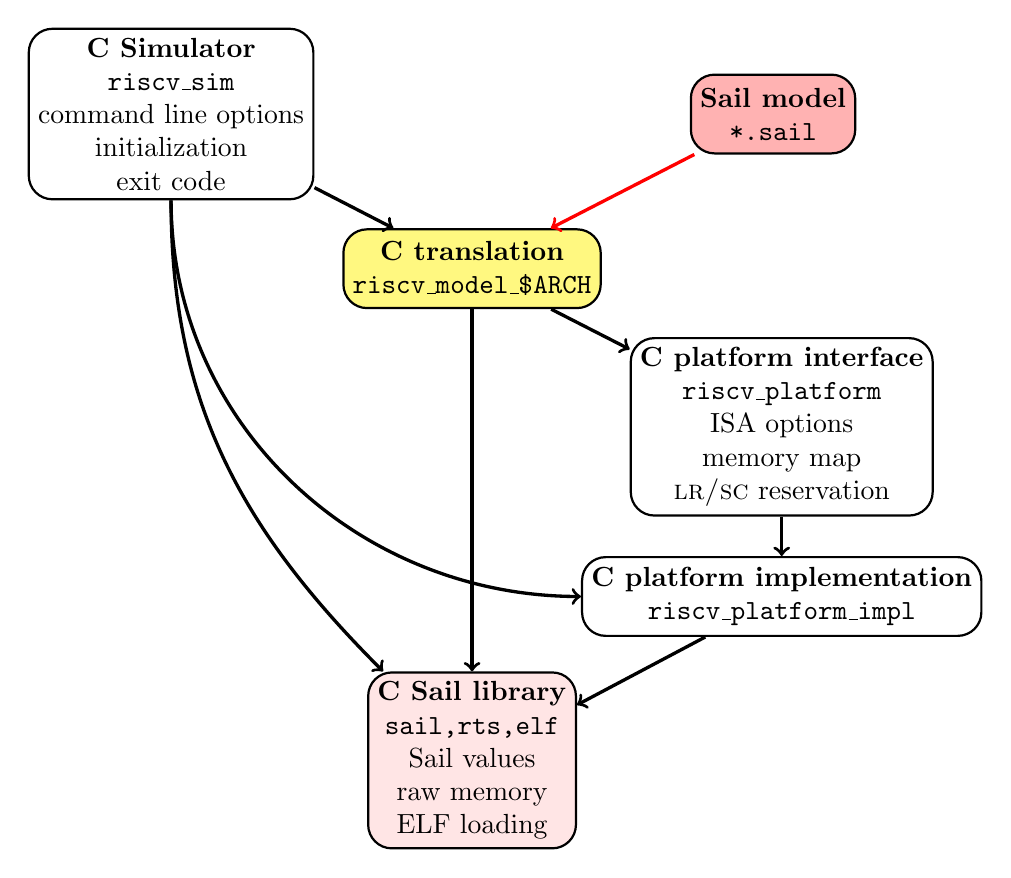
\begin{tikzpicture}[
    node distance=5mm,
    align=center,
    base/.style={rectangle, rounded corners=3mm, minimum size=10mm, thick, draw=black},
    cmodel/.style={base, fill=yellow!50},
    sail/.style={base, fill=red!30},
    c/.style={base},
    csail/.style={base,fill=red!10},
    dep/.style={black, very thick},
    gen/.style={red, very thick}
  ]

  \node (cmodel)     [cmodel]                        {\textbf{C translation}\\
                                                         \texttt{riscv\_model\_\$ARCH}};

  \node (csim)       [c, above left=of cmodel]       {\textbf{C Simulator}\\
                                                         \texttt{riscv\_sim}\\
                                                         command line options\\
                                                         initialization\\
                                                         exit code};

  \coordinate (smloc) at ($(csim)!2!(csim -| cmodel)$);
  \node (sailmodel)  [sail] at (smloc)               {\textbf{Sail model}\\
                                                         \texttt{*.sail}};

  \node (plat)       [c, below right=of cmodel]      {\textbf{C platform interface}\\
                                                         \texttt{riscv\_platform}\\
                                                         ISA options\\
                                                         memory map\\
                                                         \textsc{lr/sc} reservation};

  \node (platimpl)   [c, below=of plat]              {\textbf{C platform implementation}\\
                                                         \texttt{riscv\_platform\_impl}};

  \coordinate (clib) at ($(cmodel)!1.5!(cmodel |- platimpl)$);

  \node (csail)      [csail]  at (clib)              {\textbf{C Sail library}\\
                                                         \texttt{sail,rts,elf}\\
                                                         Sail values\\
                                                         raw memory\\
                                                         ELF loading};

  \draw[->,gen]  (sailmodel) edge                    (cmodel);

  \draw[->,dep]  (cmodel)    edge                    (plat)
                             edge                    (csail);

  \draw[->,dep]  (plat)      edge                    (platimpl);

  \draw[->,dep]  (csim)      edge                    (cmodel)
                             edge [out=-90,in=180]   (platimpl)
                             edge [out=-90,in=135]   (csail);

  \draw[->,dep]  (platimpl)  edge                    (csail);
\end{tikzpicture}
\end{document}
